\begin{circuitikz}\draw
  (0,3)to[L](1.5,3)--(1.5,2.25)to[short,o-o](1.5,0.75)--(1.5,0)--(0,0)
  (1.5,1.5)--(2,1.5)to[L](3,1.5)to[R](4,1.5)--(4.5,1.5)
  (2,1.5)--(2,2.25)to[C](4,2.25)--(4,1.5)
  (1.5,0)--(4.5,0)--(4.5,0.75)to[short,o-o](4.5,2.25)--(4.5,3)--(1.5,3)
;\end{circuitikz}  

АИР(автономный инвертор резонансный) резонансного типа.
Для нашей специальности не очень подходит. Резонансный -- значит
частоту изменить не можем.
Применяется для закалки стали.

Сокращаем количество до 8ми. Генераторы $\rightarrow$ Моторы.

\begin{tikzpicture}\draw
  (0,2)rectangle(2.5,2.8)
  (1.25,2.4) node {{\larger[2] $\sim$ $\rightarrow$ $=$}}
  (3,2)rectangle(5.5,2.8)
  (4.25,2.4) node {{\larger[2] $=$ $\rightarrow$ $\sim$}}
  (2.75,0.5)ellipse(2.7cm and 0.7cm)
  (1.8,0.5) node {\begin{tabular}{c}управляемый\\выпрямитель\end{tabular}}
  (4.1,0.5) node {\begin{tabular}{c}зависимый\\инвертор\end{tabular}};
  \draw[->](1.25,2)--++(0.75,-0.75);
  \draw[->](4.25,2)--++(-0.75,-0.75);
  ;\end{tikzpicture}

Если энергия пошла в обратную сторону. Рассмотрим управляемый выпрямитель.

НПР $\leftrightarrow$ Реверсивный выпрямитель. При одном направлении тока,
а если поставить второй транзистор. И ток и напряжение можно инвертировать.

Переменное напряжение $\sim$ -- это постоянное, которое меняется по
уровню и направлению.

$50 \sim = \sim 500$

Непосредственный -- это не 2х ступенчатый преобразователь
(преобразователь частоты со звеном постоянного тока).

Это классификация одноступенчатых преобразователей.

НПЧ -- одноступенчатый преобразователь!

Реверсивный постоянного $\leftrightarrow$ АИН. Осталось 8, но это неполная
классификация.

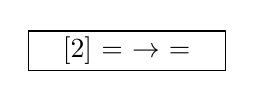
\begin{tikzpicture}
  \draw (0,-0.25)rectangle(2.5,0.25)
  (1.25,0) node {\larger[2] $=$ $\rightarrow$ $=$};
\end{tikzpicture}
-- по квадрантам.

Другие классификационные признаки, выбирается параметр, по нему
идет классификация.

2-й параметр) по типам силовых полупроводниковых приборов.

\begin{tabular}{lcl}
  неуправляемые &--&диоды \\
  управляемые &--& однозначно тиристоры
\end{tabular}

Транзисторов достаточно много. Тиристор -- отпираемые, незапираемые по
управляющему току семистор.

3-й параметр) -- тип силовой схемы.

\begin{tabular}{lcl}
нулевые схемы &--& трансформаторы с выводом ``0''-й точки.\\
мостовые& -- &содержат две нулевых.(Одна схема -- объединены катоды,\\
&&другая -- аноды)\\
кольцевые&&\\
комбинированные&&
\end{tabular}

\begin{circuitikz}\draw
  (0,2.7)--(2,2.7) node[right] {``0''} 
  (0,2) node[above] {A} to[D*](0,1)--(2,1)
  (1,2) node[above] {B} to[D*](1,1)to[short,-*](1,0.5)
  (2,2) node[above] {C} to[D*](2,1);
  \draw[<-] (1.2,0.5) -- (2.5,0.5) node[right]
  {так не говорят, что эта точка ``0''-я}
  ;\end{circuitikz}


\begin{circuitikz}\draw
  (3,0)to[D*](2,0)--(1,0)to[D*](0,0)
  (3,0.75)to[D*](2,0.75)--(1,0.75)to[D*](0,0.75)
  (3,1.5)to[D*](2,1.5)--(1,1.5)to[D*](0,1.5)
  (0,0)--(0,1.5)
  (3,0)--(3,1.5)
  (1,1.5)--(1,2) node[above] {A}
  (1.5,0.75)--(1.5,2) node[above] {B}
  (2,0)--(2,2) node[above] {C}
  (3.8, 0.75) node[right] {мостовая}
  ;\end{circuitikz}  

\begin{circuitikz}\draw
  (1,0)to[D*](2,0)
  (1,0)to[D*](0.29,0.71)
  (1,1.42)to[D*](0.29,0.71)
  (1,1.42)to[D*](2,1.42)
  (2.71,0.71)to[D*](2,1.42)
  (2.71,0.71)to[D*](2,0)
  (1,1.42)--(1,2)--(3,2)
  (2,1.42)--(2,2.4)--(0,2.4)
  (0.29,0.71)--(-.3,0.71)
  (2.71,0.71)--(3.3,0.71)
  (1,0)--(1,-0.6)--(3,-0.6)
  (2,0)--(2,-1)--(0,-1)
  ;\end{circuitikz}

4-й признак

С трансформатором или нет. Трансформатор может быть на входе и на выходе.

\begin{circuitikz}\draw
  (0,0)rectangle(2.4,0.6)
  (1.2,0.3) node {Выпрямитель}
  (1.2,0.6) node[above] {на входе}
  (3,0)rectangle(4.8,0.6)
  (3.9,0.3) node {Инвертор}
  (3.9,0.6) node[above] {на выходе}
  ;\end{circuitikz}

5-й признак -- число фаз

6-й признак -- по уровню напряжения >1000Вольт
В последних гостах по среднему уровню напряжения $6|10|35$ kV.

7-й признак -- по назначению.

\begin{tabular}{l}
для возбуждения\\
для зарядки (электрокары)\\
для гальваники
\end{tabular}

8-й признак -- по конструктивному обозначению

\begin{tabular}{lll}
  IR &--& защитная оболочка от окружающей среды\\
  &IR=0& открытое \\
  &IR=23&\\
  &IR=65& пыле-влаго
\end{tabular}

Классификация, на нее буду ссылаться

По приборам или перейти к первому типу.

\begin{tabular}{l}
  Диоды\\
  \hline\\
  обычные\\
  быстровосста-\\навливающиеся\\
  Шотки
\end{tabular}
\begin{tabular}{l}
  Тиристоры\\
  \hline\\
  обычные\\
  симметричные(симисторы)\\
  запираемые\\
\end{tabular}
\begin{tabular}{l}
  Транзисторы\\
  \hline\\
  биполярные\\
  униполярные\\
  pn переходом\\
  с изолированным затвором\\
  со встроенным\\
  с индуцированным
\end{tabular}

Варисторы, стабилитроны(кремнивые ограничители). Везде делается акцент
на большую мощность.

9-й признак -- диапазон мощности современных устройств от зарядки
телефона, до линий передач постоянным током $10^4$, была линия $10^5$ Вольт.

\begin{tabular}{ll}
  $U$& $10^0$..$10^4$В\\
  $I$& $10^{-2}$..$10^4$А\\
  $P$& $10^{-1}$..$10^6$-$10^7$Вт\\
  $T$& 0;0..50,100,200,400Гц..$10^4$ ($10^5$Hz)
\end{tabular}

$10^5$ используется несущая частота, а не рабочая частота.
--- доли микрогенри, 1MGz -- это сопротивление значительное.

\section{Выпрямители}
Установки большой мощности всегда трехфазные. В квартирах разводятся так,
чтобы напряжение было приблизительно одинаковые в среднем для разных фаз.
Будем использовать однолинейное изображение многофазных сетей

\begin{circuitikz}\draw
  (0,1.5)--(0,1)to[C](0,0)
  (-0.3,0)--(0.3,0)
  (-0.1,0.9)--(0.1,1.1)
  (-0.1,1)--(0.1,1.2)
  (-0.1,1.1)--(0.1,1.3)
  (1,0.75) node {{\larger[3] =}}
  (2,1.5)to[C](2,0.5)
  (2.75,1.5)to[C](2.75,0.5)
  (3.5,1.5)to[C](3.5,0.5)
  (2,0.5)--(3.5,0.5)
  (2.75,0.5)--(2.75,0)
  (2.45,0)--(3.05,0)
  (6,1.5)--(6,1)to[C](6,0)
  (5.9,1)--(6.1,1.2) node[right] {12}
  (5.7,0)--(6.3,0)
  ;\end{circuitikz}

\begin{tabular}{cl}
  $U$ & $u=f(t)$\\
  $E$ & e\\
  $I$ & i
\end{tabular}

$I$ -- действующее или среднеквадратичное значение. Постоянное по направлению и есть
пульсации.

\begin{tikzpicture}
  \draw[thin,->] (0,0)--(0,2.3);
  \draw[thin,->] (0,0)--(4,0);
  \draw[domain=0.1:4.7,smooth]
  plot(\x,{1.6 + 0.1*sin((10*\x) r)});
  \draw[<->] (1,0.1)--(1,1.45) node[midway,left] {$I_d$};
  \draw[<->] (2.2,0.1)--(2.2,1.45) node[midway,right] {$i_d$};
  \draw[<-] (2.8,0.8)--(4.2,1.2) node[right] {direct -- прямое, выпрямленное};
  \draw(4.2,0.7) node[right] {для постоянного тока большая буква $I_d$}
;\end{tikzpicture}

\begin{circuitikz}\draw
  (0,0)rectangle(1.5,1)
  (0.75,0.5) node {F}
  (0,1.8)rectangle(1.5,2.6)
  (1.25,2.2)to[Ty](0.25,2.2)
  (0.75,2.6)--(0.75,3.15)
  (0.2,1)--(0.2,1.8) node[midway,left] {{\larger[2] +}}
  (1.3,1)--(1.3,1.8) node[midway,right]{{\larger[2] --}}
  (0.75,3.6) circle(0.45)
  (0.75,4.05) circle(0.45)
  (0.75,4.5)--(0.75,5.3)--(0.25,5.8)
  (0.65,5.4)--(0.55,5.3)--(0.35,5.5)--(0.45,5.6) %выключатель
  (0.75,5.6) node[right] {$QF_1$ -- переменного тока}
  (0.65,4.7)--(0.85,4.9)
  (0.65,4.8)--(0.85,5)
  (0.65,4.9)--(0.85,5.1)
  (0.75,5.8)--(0.75,6.3)
  (-0.4,6.3)--(1.5,6.3)
  (-0.1,6.2)--(0.1,6.4)
  (0,6.2)--(0.2,6.4)
  (0.1,6.2)--(0.3,6.4)

  (1.5,0.8)--(2.5,0.8)--(3,1.3)
  (3.1,0.9) node[above right] {$QF_2$ -- постоянного тока}
  (2.6,0.9)--(2.5,1.0)--(2.7,1.2)--(2.8,1.1) % выключатель
  (3,0.8)--(4.5,0.8)to[european resistor, bipoles/length=1.5cm](6.3,0.8)
  (1.5,0.2)--(6.3,0.2) --(6.3,0.8)
  (1.5,0.2) node[below right] {\larger[2] +}
  (1.5,0.8) node[above right] {\larger[2] --}

  (8,5) to[ospst,l_={S -- switch}] (8,6)
  (7.3,4.2) node[right] {QF -- в силовых цепях}
  (7.5,3.5)to[european resistor](8.5,3.5) node[right] {R}
  (7.5,2.8)--(8,2.8)--(8,3.05)arc(90:360:0.25)--(8.5,2.8) node[right] {L}
  (7.5,2.1)to[C](8.5,2.1) node[right] {C}
  (7.5,1.4)to[battery1](8.5,1.4) node[right] {B}
  (7.5,0.7)to[fuse](8.5,0.7) node[right] {F}

  (-1.7,1.6)rectangle(-0.2,3)
  (-0.95,2.3) node {СУВ}
  ;\end{circuitikz}  

\begin{circuitikz}\draw
  (0,0) node[right] {${\displaystyle C= \varepsilon\frac{S}{d}}$};
  \draw[<-] (1.6,0.3)--(2.4,0.5) node[right] {большое};
  \draw[<-] (1.6,-0.2)--(2.4,-0.2) node[right]
       {\begin{tabular}{c}малое\\пленка\end{tabular}};
  ;\end{circuitikz}  

Электролитический конденсатор пропитан проводящим раствором, создается пленка.
Выключатели по включению по часовой стрелке.
Трансформаторы рисуют так:

\begin{circuitikz}\draw
  (0,1)to[L](0,0)
  (0.75,1)to[L](0.75,0)
  (1.5,1)to[L](1.5,0)
  (0,1)--(1.5,1)
  (0,1.5)--(1.5,1.5)
  (0,1.24)rectangle(1.5,1.26)
  (0,2.5)to[L](0,1.5)
  (0.75,2.5)to[L](0.75,1.5)
  (1.5,2.5)to[L](1.5,1.5)
  ;\end{circuitikz}

VB -- выпрямительный блок. На выходе выпрямителя есть фильтр.

СУВ -- система управления выпрямителя, включает в себя диагностику, измерения,
сигнализацию, контроль, защиты.

Назначение трансформатора:
\begin{itemize}
\item T -- изменяет уровни напряжения
  $$
  U_1 \rightarrow U_2
  $$
\item T -- преобразование числа фаз.
  $$
  m_2 \rightarrow m_1
  $$
\item гальваническая развязка
\item сопротивление К.З.; ограничение тока короткого замыкания Т.К.З. Электрические
  аппараты должны быть устойчивы к токам К.З. Чтобы К.З. не развивалось. Не должно
  приводить к выводу других приборов.

  Есть термическое, динамическое, всё это $I^2_\textcyrillic{КЗ}$.

  $I_\textcyrillic{КЗ}=100$, нагрев $10^4$

  Специальные токоограничивающие реакторы.

  $I_\textcyrillic{КЗ}\approx$ кратен $I_\textcyrillic{ном}$ $5..10..15$ раз.

  Рассмотрим производственное помещение, превышение  $5..10..15$ раз в трансформаторе,
  а для станков это много.
\end{itemize}

T, вернее его $R$ -- естественный ограничитель, в некоторых случаях можно выбросить.
Если нужен только токоограничитель, то ставим токоограничивающий реактор.

\begin{circuitikz}\draw
  (0,0)--(0,0.35)arc(270:0:0.35)--(0,0.7)--(0,2)
  (-0.1,1.2)--(0.1,1.4)
  (-0.1,1.3)--(0.1,1.5)
  (-0.1,1.4)--(0.1,1.6)
  ;\end{circuitikz}

СУВ = СИФУ -- система импульсно-фазового управления. Реализуется теми же программными
средствами в микроконтроллере. выходной сигрнал. через усилитель мощности
подается сигнал.


Фильтр: Всегда задаю вопрос, что такое

\begin{tabular}{ccc}
  R &--& коэффициэнт пропорциональности ${\displaystyle \frac{U}{I}}$\\
  L & --& коэффицэнт пропорциональности ${\displaystyle \frac{\Psi}{I} =
    \frac{\omega \Phi}{I}}$\\
  C &--&${\displaystyle \frac{q}{U}}$
\end{tabular}

Любая из этих величин философская, физическая.
R -- это потери! В нашем случае КПД на первом месте!
\begin{itemize}
\item L
\item C
\item L--C
\item C--L Г-образная
\item C--L--C Т-образная  
\end{itemize}

Основные характеристики фильтра:
Во сколько раз снижается пульсаций.

\begin{circuitikz}\draw
  (0,2)--(2,2)to[L,l={L}](3,2)--(5,2)to[R,l={$R_\textcyrillic{н}$}](5,0)--(0,0)
  (0,1) node {\begin{tabular}{c}U\\u\end{tabular}}
  (2.5,1) node {$U_c + u^\prime$};
  \draw[<->](4,2)--(4,0) node[midway,left] {$u^{\prime\prime}$}
  ;\end{circuitikz}

Обмотка возбуждения генератора это хорошо?

Коэффициэент сглаживания фильтра
${\displaystyle К= \frac{u^{\prime\prime}}{u^\prime}}$

$$
Z = \sqrt{R^2_\textcyrillic{н} + (\omega L)^2}
$$

Отсюда коэффициент сглаживания фильтра =

$K={\displaystyle \frac{u^\prime}{\frac{u^\prime}{z}R_\textcyrillic{н}}}$ =
${\displaystyle \frac{Z}{R_\textcyrillic{н}}} = \sqrt{1 +(\omega T)^2}
\approx \omega T$, при $\omega T = 4$

C-фильтр

\begin{circuitikz}\draw
  (0,2)--(2,2)
  (0,0)--(2,0)
  (1,0)to[C](1,2)
   ;\end{circuitikz}

Пульсация до установки на пульсацию после.
Фильтр будет хорошо действовать когда будут диоды, будет их запирать.

Коэффициэнт сглаживания фильтров -- самостоятельно. Зарисовать схемы.

Это классические реактивные фильтры. Существуют резонансные фильтры.

\begin{circuitikz}\draw
  (0,1.5)--(0.5,1.5)--(0.5,1.15)to[C](1.5,1.15)--(1.5,1.5)
  (0.5,1.5)--(0.5,1.85)to[L](1.5,1.85)--(1.5,1.5)--(2,1.5)
  to[L](2,0.75)to[C](2,0)
  (2,1.5)--(2.75,1.5)to[european resistor](2.75,0)--(0,0);
  \draw[<-] (2.1,0.2)--(3,0) node[right] {для остальных частот добавим} 
  ;\end{circuitikz} Фильтр-пробка  
$$
\omega_\textcyrillic{рез} = \frac{1}{\sqrt{LC}}
$$
Теоретически задержит полностью. Он эффективен только на одной частоте.
$\omega_\textcyrillic{рез}$ -- здесь на резонансной частоте сопротивление 0

В последнее время применяют активные фильтры.

Активный генератор переменной составляющей:

\begin{circuitikz}\draw
  (0,2)to[L](2,2)--(2,1.5)
  (1.5,0.5)rectangle(2.5,1.5)
  (2,1) node {АФ}
  (0,0)--(2,0)--(2,0.5)
  (2,2)--(3.5,2)to[european resistor](3.5,0)--(2,0)
  (1,2.3)node {$i_d$};
  \draw[->](1.3,2.3)--(3.2,2.3);
  \draw[<-] (2.6,1.6)--(3.7,2) node[right]
       {\begin{tabular}{c}в противовазе добавляем\\
           $i^\prime=i^{\prime\prime}$\end{tabular}}
       ;\end{circuitikz}

Это тоже что и резонансный фильтр, но <имеет собственный
источник энергии>. Это тоже преобразователь.

Д.з. -- транзисторы и фильтры.
